\documentclass[a4paper]{article}
\usepackage{fullpage} % Good use of white space, reduces number of pages -> less stressed students :-)
\usepackage[fancy]{template} % Setup for headers

% \usepackage[solution]{written-exam}  % Show with solutions
\usepackage{../written-exam}        % Show without solutions

\usepackage{listings}             % Include the listings-package
\usepackage{todonotes}            % Good for comments
% \renewcommand{\todo}[1]{}  % Uncomment to remove todonotes

\usepackage{arydshln}
\usepackage{xstring} % For string indexing.

\usepackage{tikz}
\usetikzlibrary{shapes,arrows,fit,calc,positioning}
\usepackage{scalefnt}

\usepackage{nameref}
\usepackage{remreset}

%% Details about the exam
\setup{%
  subject={\textbf{Date:} April 17, 2018},%
  assignment={4-hour Written Re-Exam in Computer Systems},%
  date={}%
}
\setupLocation[short=DIKU]{
  Department of Computer Science, University of Copenhagen%
}

\begin{document}
\pagenumbering{roman}

\maketitle

% !TEX root = master.tex


\section*{Preamble}
\addcontentsline{toc}{section}{Preamble}

\begin{solution}
\emph{Disclaimer:} The reference solutions in the following range from exact results to sketch solutions; this is entirely on purpose. Some of the assignments are very open, which reflects to our solutions being just one of many. Of course we try to give a good solution and even solutions that are much more detailed than what we expect you to give. On the other hand, you would expect to give more detailed solutions that our sketches. Given the broad spectrum of solutions, it is not possible to directly infer any grade level from this document. \textcolor{solutioncolor}{All solutions have been written in the in-lined space with this colour.}
\end{solution}

This is the text is an excerpt of the exam set for the 4 hour written re-exam in Computer Systems (CompSys), B1+2-2017/18.
This document consists of \pageref{LastPage} pages excluding this preamble; make sure you have them all. Read the rest of this preamble carefully. 
Your submission will be graded as a whole, on the 7-point grading scale, with external censorship.

\begin{itemize}
  \item You can answer in either Danish or English.
  \item Remember to write your exam number on all pages.
  \item You do not have to hand-in this preamble.
\end{itemize}

\subsection*{Expected usage of time and space}
The set is divided into sub-parts that each are given a rough guiding estimate of the time needed. However, your exact usage of time can differ depending on prior knowledge and skill.

Furthermore, all questions includes formatted space (lines, figures, tables, etc.) for in-line answers. Please use these as much as possible. The available spaces are intended to be large enough to include a satisfactory answer of the question; thus, full answers of the question does not necessarily use all available space.
\\
If you find yourself in a position where you need more space or have to redo (partly) an answer to a question, continue on the backside of a paper or write on a separate sheet of paper. Ensure that the question number is included and that you in the in-lined answer space refers to it; e.g. write ``\emph{The [rest of this] answer is written on backside of/in appended page XX.}''

For the true/false and multiple-choice questions with one right answer give only one clearly marked answer. If more answers are given, it will be interpreted as incorrectly answered. Thus, if you change your answer, make sure that this shows clearly.


\subsection*{Exam Policy}
This is an \emph{individual}, open-book exam.
You may use the course book, notes and any documents printed or stored on your computer, but you may not search the Internet or communicate with others to answer the exam.

\subsection*{Errors and Ambiguities}

In the event of errors or ambiguities in the exam text, you are expected to
state your assumptions as to the intended meaning in your answer.
%
Some ambiguities may be intentional.




\pagebreak
\pagenumbering{arabic}
\setcounter{page}{1}

% !TEX root = master.tex

\lstdefinelanguage
   [x64]{Assembler}     % add a "x64" dialect of Assembler
   [x86masm]{Assembler} % based on the "x86masm" dialect
   % with these extra keywords:
   {morekeywords={CDQE,CQO,CMPSQ,CMPXCHG16B,JRCXZ,LODSQ,MOVSXD, %
                  POPFQ,PUSHFQ,SCASQ,STOSQ,IRETQ,RDTSCP,SWAPGS, %
                  TESTQ, MOVQ, ADDQ, SUBQ, CMPQ, CMOVQ, LEAQ, CMOVG, MOVL, negq, cmovs, sarq, cmovl, imulq, pushq, popq,%
                  rax,rdx,rcx,rbx,rsi,rdi,rsp,rbp, %
                  r8,r8d,r8w,r8b,r9,r9d,r9w,r9b}}

\lstset{language={[x64]Assembler}}

\questionhead{Machine architecture}{80 minutes}

\subquestionhead{True/False Questions}{8 minutes}
\begin{tfquestion}
\tfitem[false]{Within Boolean arithmetic then ${\tilde{\;}\,}( A \;\&\; B) = ({\tilde{\;}\,} A)\; \hat{\;} \;({\tilde{\;}\,} B)$.}
\tfitem[false]{The largest \lstinline{unsigned char} has the value 256.}
\tfitem[true]{The lowest \lstinline{signed char} has the value -128.}
% \tfitem{In the IEEE floating point format, a value is denormalised if the exponent is different from 0.}
\tfitem[false]{Assume \lstinline{x} and \lstinline{y} are signed natural values (e.g. \lstinline{long}), then the C expression \lstinline{(x < y) == ((-x) > (-y))} is always evaluated to true.}
\tfitem[false]{In the Linux call model, the return address of a procedure call is located in a special purpose register.}
\end{tfquestion}
\ifsolution{a) is false, though is looks like DeMorgan's law. Write truth table or consider the size of the domains.}

\noindent
\ifsolution{d) is false as the arithmetic negation of the smallest (negative) value of a two's complement number does not have positive representative. Thus for this number then \lstinline{x == -x}.}

\noindent
\ifsolution{e) is false as the return address is located on the stack.}

\subquestionhead{Multiple Choice Questions}{8 minutes}
\emph{In each of the following questions choose one answer.}

\begin{mcquestion}
In a pipelined architecture, resolving correctness of a predicted jump is performed in the:
\mcitem{Fetch phase (\lstinline{F}),}
\mcitem{decode phase (\lstinline{D}),}
\mcitem[check]{execute phase (\lstinline{X}), or}
\mcitem{memory phase (\lstinline{M}).}
\end{mcquestion}

\begin{mcquestion}
The 6-bit two's complement number \lstinline{100101} represents the value
\mcitem{37,}
\mcitem{27,}
\mcitem{17,}
\mcitem{-17,}
\mcitem[check]{-27, or}
\mcitem{-37.}
\end{mcquestion}

% \begin{mcquestion}
% Consider the following C program for calculating the sum of the entries of a 2-D array.
% \begin{lstlisting}[language={C}]
% long arr_sum (long a[M][N]) {
%   int sum;
%   for (int i = 0; i < M; i++) {
%     for (int j = 0; j < N; j++) {
%       sum += a[i][j];
%     }
%   }
%   return sum;
% }
% \end{lstlisting}
% How would you characterise the behaviour of the program with respect to locality of execution?
% \mcitem{Only good temporal locality.}
% \mcitem{Only good spacial locality.}
% \mcitem[check]{Both good spacial and temporal locality.}
% \mcitem{Neither good spacial nor temporal locality.}
% \end{mcquestion}

% Block offset size: log_2(32) = 5 bits
% Set index size: log_2(16*1024/32/4) = 7 bits
% Tag size = 64-5-7 = 52

% \begin{mcquestion}
% Given a byte-addressed machine with 64-bit addresses, that is equipped with a 4-way set-associative data cache of 16 kilobytes and a block size of 32 bytes. How many bits are used for the tag?
% \mcitem{32 bits}
% \mcitem{40 bits}
% \mcitem{46 bits}
% \mcitem{52 bits}
% \mcitem{58 bits}
% \end{mcquestion}

% % Block offset size: log_2(32) = 5 bits
% % Set index size: log_2(16*1024/32/4) = 7 bits
% % Tag size = 64-5-7 = 52


\newpage
\subquestionhead{Data Cache}{16 minutes}

Given a byte-addressed machine with 16-bit addresses.
The machine is equipped with a 4-way set associative data cache of 8 kilobytes.
Cache have a block size of 16 bytes.

% \textbf{Løsning} \\
% Da blokken er 16 bytes bruges 4, bit (0-3) til at indexere indenfor blokken
% Da cachen er 8Kb og blok størrelsen er 16 bytes er der 512 blokke i cachen.
% Da cachen er 4-vejs associativ er der 128 "sets" i cachen. Der kræves 7 bit
% for at vælge sæt (bits 4-10).
% Resten er "tag" (bits 11-15).
% \textbf{Løsning slut}
% }

\begin{question}
For each bit in the table below, indicate which bits of the address would be used for
\begin{itemize}
  \item block offset (denote it with \texttt{O}),
  \item cache tag (denote it with \texttt{T}), and
  \item set index (denote it with \texttt{S}).
\end{itemize}

\begin{center}
    \renewcommand{\arraystretch}{1.8}
\begin{tabular}{cccccccccccccccc}
\hline
 \multicolumn{1}{|p{5mm}|}{\ifsolution{\texttt{T}}}
& \multicolumn{1}{p{5mm}|}{\ifsolution{\texttt{T}}}
& \multicolumn{1}{p{5mm}|}{\ifsolution{\texttt{T}}}
& \multicolumn{1}{p{5mm}|}{\ifsolution{\texttt{T}}}
& \multicolumn{1}{p{5mm}|}{\ifsolution{\texttt{T}}}
& \multicolumn{1}{p{5mm}|}{\ifsolution{\texttt{S}}}
& \multicolumn{1}{p{5mm}|}{\ifsolution{\texttt{S}}}
& \multicolumn{1}{p{5mm}|}{\ifsolution{\texttt{S}}}
& \multicolumn{1}{p{5mm}|}{\ifsolution{\texttt{S}}}
& \multicolumn{1}{p{5mm}|}{\ifsolution{\texttt{S}}}
& \multicolumn{1}{p{5mm}|}{\ifsolution{\texttt{S}}}
& \multicolumn{1}{p{5mm}|}{\ifsolution{\texttt{S}}}
& \multicolumn{1}{p{5mm}|}{\ifsolution{\texttt{O}}}
& \multicolumn{1}{p{5mm}|}{\ifsolution{\texttt{O}}}
& \multicolumn{1}{p{5mm}|}{\ifsolution{\texttt{O}}}
& \multicolumn{1}{p{5mm}|}{\ifsolution{\texttt{O}}}\\
\hline
15&14&13&12&11&10&9&8&7&6&5&4&3&2&1&0\\
\end{tabular}
\end{center}
\end{question}

\begin{question}
Consider the stream of storage references in hexadecimal format: 
\begin{quotation}
  \texttt{0xA010}
, \texttt{0xF020}
, \texttt{0xFF20}
, \texttt{0xFF0C}
, \texttt{0x0028}
, \texttt{0xF0A4}
, \texttt{0xF034}
.
\end{quotation}

\noindent Assuming that the cache initially is cold followed by referencing the above stream. Given that the cache uses LRU replacement, what is the effect of a following reference to address: \hspace{5mm}\textbf{\texttt{0x0024}}.

\begin{center}
    \renewcommand{\arraystretch}{1.8}
\begin{tabular}{|l|p{5cm}|}
\hline
Block Offset: & \texttt{0x}\ifsolution{\texttt{4}}\\
\hline
Set Index:    & \texttt{0x}\ifsolution{\texttt{02}}\\
\hline
Cache tag:    & \texttt{0x}\ifsolution{\texttt{00}}\\
\hline
Cache hit or miss:    & \ifsolution{hit} \\
\hline
In case of cache miss, which cache tag is evicted: & \\
\hline
\end{tabular}
\end{center}
\end{question}

\begin{question}
Briefly argument for your answer regarding cache hit/miss and address eviction and show the content of the set before and after the reference.

\answerlines[The address is already in the cache as the block containing it was loaded with \texttt{0x0028}. The cache is 4-way and the only other following block loaded into the same set \texttt{0x01} is \texttt{0xF034}.]{8}
\end{question}

\newpage


\subquestionhead{Assembler programming}{30 minutes}

Consider the following program written in X86-assembler.

\begin{lstlisting}[language={[x64]Assembler}, numbers=left]
program:
  movq  %rdi, %rax
  movl  $0, %edx
  jmp L2
L3:
  addq  (%rax), %rdx
  addq  $8, %rax
L2:
  cmpq  %rsi, %rdx
  jl  L3  
  subq  %rdi, %rax
  sarq  $2, %rax
  ret
\end{lstlisting}

\begin{question}
Rewrite the above X86-assembler program to a C program and explain the functionality of the program. The resulting program should not have a goto-style and minor syntactical mistakes are acceptable.
\answerlinesfill[
The program take two arguments (\lstinline{\%rdi} and \lstinline{\%rsi}) and calculates twice the number of elements in an unbounded array (*a) that is a required to reach max.\\
~\\
\lstinline{long program(long *arr, long max) \{}\\
\lstinline{\ \ long *arr_ptr = arr; // Located in \%rdi}\\
\lstinline{\ \ long sum = 0; // Located in \%rdx}\\
\lstinline{\ \ while (sum < max) \{}\\
\lstinline{\ \ \ \ sum += *arr_ptr;}\\
\lstinline{\ \ \ \ arr_ptr++;}\\
\lstinline{\ \ \}}\\
\lstinline{\ \ return (arr_ptr - arr) * 2;}\\
\lstinline{\}}\\
~\\
That the return values was twice the size was unintended and due to a copy-paste error; the instruction should have right-shifted by 3. Any answer that does not include this is also accepted and this part should show understanding of pointer arithmetic.
]
\end{question}

\begin{question}
Argument for your choice of statements and expression. Specify which part of the program are not directly translated and argue why.
\answerlines[We see on the register types that values are \lstinline{long}.
First argument (\lstinline{\%rdi} which is used in \lstinline{\%rax}) is a pointer to an array; this is seen by the indexing in line 6. The second (\lstinline{\%rsi}) is a number. \lstinline{\%rdx} is overwritten by 0 (in \lstinline{\%edx}) and therefore not an input.\\
The program structure is a standard while loop as following translation from BOH.
The comparison of \lstinline{\%rsi} to \lstinline{\%rdx} with the following jump-less-than is the condition of \lstinline{sum} < lstinline{max}.\\
The array is iterated using pointer arithmetic which is seen in line 7. Line 11 finds the number of elements from the initial array pointer, which in line 12 is divided by 4 using a right-shift. (Note, this was intended to be 8 (shift 3) to account for the length a \lstinline{long}; thus the return value is twice the length.)
]{12}
\end{question}


\begin{question}
Briefly describe the semantic difference between logical and arithmetical shifts.
\answerlines[Right shifts are identical. A logical left shift always adds a 0 as the most significant bit. Arithmetical left shifts duplicated the most significant bit to ensure the sign of a two's complement number.]{5}

\end{question}



\pagebreak

% !TEX root = master.tex

% Questions and answers by Troels Henriksen

\questionhead{Operating Systems}{80 minutes}
\lstset{language=C}

\subquestionhead{True/False Questions}{8 minutes}

\begin{tfquestion}
\tfitem[true]{\lstinline{fopen()} is not a system call.}
\tfitem[false]{There is never more physical memory than virtual memory.}
\tfitem[false]{System calls are implemented via signals.}
\tfitem[false]{Virtual memory requires a disk.}
\tfitem[false]{System calls run in user mode.}
\tfitem[true]{Condition variables cannot be efficiently implemented solely with mutexes.}
\end{tfquestion}

\subquestionhead{Multiple Choice Questions}{12 minutes}
\emph{In each of the following questions, you may put one or more answers.}

\begin{mcquestion}
Which of the following operations are guaranteed to execute atomically?

\mcitem{\texttt{pthread\_cond\_signal()}}
\mcitem[check]{\texttt{pthread\_mutex\_lock()}}
\mcitem{\texttt{x++} (when \texttt{x} is \texttt{int})}
\mcitem{\texttt{memcpy(\&x, \&y, sizeof(x))}}
\mcitem[check]{\texttt{pthread\_cond\_wait()}}
\mcitem{\texttt{exit(0)}}
\end{mcquestion}

\begin{mcquestion}
Consider a demand-paged system with the following time-measured utilisations:

  \begin{tabular}{lr}
    CPU utilisation & 50\% \\
    Paging disk & 0.7\% \\
    Other I/O devices & 75\%
  \end{tabular}

\noindent Which of the following would likely improve CPU utilisation?

\mcitem[check]{Install a faster CPU.}
\mcitem{Install a bigger paging disk.}
\mcitem{Install a faster paging disk.}
\mcitem{Install more main memory.}
\mcitem[check]{Increase the degree of multiprogramming.}
\end{mcquestion}

\newpage
\subquestionhead{Long Questions}{36 minutes}

\begin{question}
  Which of the following programming techniques and data structures
  are ``good'' for a demand-paged environment, and which are ``bad''
  (performance-wise)?  Explain your answers.

  \begin{itemize}
  \item Stack
  \item Hash table
  \item Sequential search of array
  \item Sequential search of linked list
  \item Binary search of array
  \item Vector operations (such as vector addition or computing dot products)
  \end{itemize}

  \answerlinesfill[A stack is efficient because operations exhibit
  good \textit{locality}---we are always operating on addresses near
  each other, which minimises page faults.  A hash table can be
  inefficient, because a good hash algorithm will ensure that accesses
  are evenly distributed among buckets.  A sequential search of an
  array is efficient, because of good locality.  Sequentially
  searching of a linked list is likely inefficient, because logically
  neighboring nodes can be arbitrarily distant in memory.  Binary
  search of an array is likewise also inefficient (from a memory
  access point of view), again because of large jumps in addresses.
  Vector operations tend to be efficient, because they involve
  sequentially traversing arrays.]
\end{question}

% \answerfigure


\pagebreak

% !TEX root = master.tex

% Questions and answers by Vivek Shah

\questionhead{Computer Networks}{80 minutes}
\subquestionhead{True/False Questions}{8 minutes}
\begin{tfquestion}
\tfitem[true]{Implementation of link layer protocols span both hardware (network controllers) and software (operating systems).}
\tfitem[true]{Peer-to-peer architectures exhibit better scalability because adding peers results in an increase in cumulative bandwidth available for all communicating parties.}
\tfitem[false]{For a TCP connection, the receive window can never become zero.}
\tfitem[true]{Convergence time of OSPF protocol is independent of the number of edges in a network.}
\end{tfquestion}

\subquestionhead{Multiple Choice Questions}{15 minutes}
\emph{In each of the following questions choose one answer.}

\begin{mcquestion}
Consider a two dimensional even parity scheme for error detection. Using this scheme compute the parity bits of the 8-bit ASCII\footnote{ASCII codes of A-Z lie contiguously between decimal numbers 65-90.} representation of "REEXAM" where each byte of the word forms a row for the two dimensional parity scheme. The resultant parity bits (row followed by column parity bits) are
\mcitem[check]{111100 00000110}
\mcitem{111101 00000010}
\mcitem{100101 00001110}
\mcitem{None of the above}
\end{mcquestion}

\begin{mcquestion}
The broadcast address of the network 117.18.31.54/18 is 
\mcitem{117.18.31.255}
\mcitem[check]{117.18.63.255}
\mcitem{117.18.127.255}
\mcitem{None of the above}
\end{mcquestion}

\clearpage 
\subquestionhead{Short Questions}{24 minutes}

\begin{question}
Why is an ARP query sent within a broadcast frame while the ARP response is sent within a frame having a specific destination address?
\vspace{-2ex}
\answerlines[An ARP query is sent to resolve an IP address to a
MAC address by the link layer. Since the destination MAC address
is unknown, a link layer frame consisting of the ARP query is
broadcast using the special MAC broadcast address. Since an ARP
response is sent on receipt of an ARP query which contains the MAC
address of the sender, the link layer frame containing the ARP
response can be sent to the specific MAC address of the ARP query sender.]{12}
\end{question}

\clearpage

\subquestionhead{Network Routing}{18 minutes}
Consider the network topology outlined in the graph below

\begin{center}
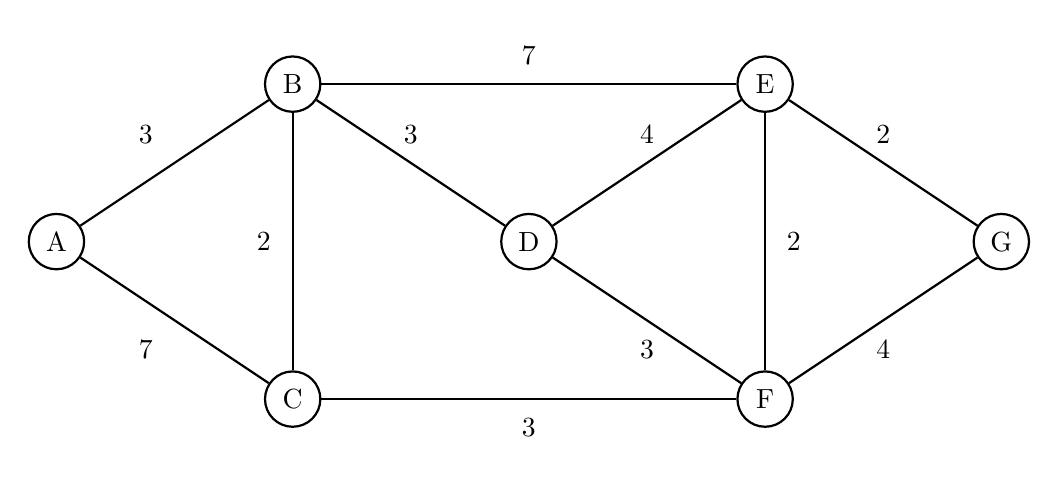
\begin{tikzpicture}[thick,minimum size=20pt,]
    \node[shape=circle,draw=black] (A) at (0,0) {A};
    \node[shape=circle,draw=black] (B) at (3,2) {B};
    \node[shape=circle,draw=black] (C) at (3,-2) {C};
    \node[shape=circle,draw=black] (D) at (6,0) {D};
    \node[shape=circle,draw=black] (E) at (9,2) {E};
    \node[shape=circle,draw=black] (F) at (9,-2) {F};
    \node[shape=circle,draw=black] (G) at (12,0) {G};
    \path [-](A) edge node[above left]{$3$} (B);
    \path [-](A) edge node[below left]{$7$} (C);
    \path [-](B) edge node[left]{$2$} (C);
    \path [-](B) edge node[above]{$3$} (D);
    %\path [-](C) edge node[below]{$4$} (D);
    \path [-](D) edge node[above]{$4$} (E);
    \path [-](D) edge node[below]{$3$} (F);
    \path [-](B) edge node[above]{$7$} (E);
    \path [-](C) edge node[below]{$3$} (F);
    \path [-](E) edge node[above]{$2$} (G);
    \path [-](E) edge node[right]{$2$} (F);
    \path [-](F) edge node[below]{$4$} (G);
\end{tikzpicture}
\end{center}

\begin{question}
Apply the link state routing algorithm and compute the forwarding tables on nodes A and D. (Note: Remember to show the steps of the algorithm.)\\
\answerfigure[The computation of link state routing algorithm
on node A:\\ \\
\begin{tabular}{|c|c|c|c|c|c|c|c|}
\hline
  Step & N' & D(B),p(B) & D(C),p(C) & D(D),p(D) & D(E),p(E) & D(F),p(F) & D(G),p(G) \\ \hline
  0 & A & 3,A & 7,A & $\infty$ & $\infty$ & $\infty$ & $\infty$ \\ \hline
  1 & AB &  & 5,B & 6,B & 10,B &  &  \\ \hline
  2 & ABC &  &  &  &  & 8,C &  \\ \hline
  3 & ABCD &  &  &  & 10,D/B & 8,C & \\ \hline
  4 & ABCDF &  &  &  & 10,D/B/F &  & 12,F \\ \hline
  5 & ABCDFE & & & & & & 12,F/E \\ \hline
  6 & ABCDFEG & & & & & & \\ \hline
\end{tabular}\\ \\
In the above computation, if there are multiple paths with same
cost they have been shown with / to demarcate them being
acceptable values. \\ \\
The computation of link state algorithm on node D:\\ \\
\begin{tabular}{|c|c|c|c|c|c|c|c|}
\hline
  Step & N' & D(A),p(A) & D(B),p(B) & D(C),p(C) & D(E),p(E) & D(F),p(F) & D(G),p(G) \\ \hline
  0 & D & $\infty$ & 3,D & $\infty$ & 4,D & 3,D & $\infty$ \\ \hline
  1 & DB & 6,B &  & 5,B & 4,D &  &  \\ \hline
  2 & DBF &  &  & 5,B & 4,D & & 7,F \\ \hline
  3 & DBFE &  &  &  &  & 3,D & 6,E \\ \hline
  4 & DBFEC & 6,B &  &  &  &  &  \\ \hline
  5 & DBFECA & & & & & & \\ \hline
  6 & DBFECAG & & & & & & \\ \hline
\end{tabular}\\ \\
In the above computation because of equal cost paths existing the
choice of nodes in N' can be inverted in step 1 and 2 and in steps
5 and 6.]{14cm}
\answerfigure[Forwarding table on node A follows:\\ \\
\begin{tabular}{|c|c|}
  \hline
  Destination node & Edge \\ \hline
  all nodes & (A,B) \\ \hline
\end{tabular} \\ \\ \\ \\
Forwarding table on node D follows:\\ \\
\begin{tabular}{|c|c|}
  \hline
  Destination node & Edge \\ \hline
  A & (D,B) \\ \hline
  B & (D,B) \\ \hline
  C & (D,B) \\ \hline
  E & (D,E) \\ \hline
  F & (D,F) \\ \hline
  G & (D,E) \\ \hline
\end{tabular}]{10cm}
\end{question}

\begin{question}
List the problems that are overcome using hierarchical routing.
\vspace{-3ex}
\answerlines[Some of the problems that are solved by hierarchical
routing are: \\
1. Scalability issues in message communication overheads with
growing network size.\\
2. Scalability issues in routing algorithm computing overheads
with growing network size.\\
3. Scalability issues in storage and retrieval overheads of
routing information with growing network size. \\
2. Administrative autonomy which allows each autonomous network to
operate and administer itself while still being able to
inter-operate with other networks.]{12}
\end{question}




\end{document}
